%\documentstyle[graphicx,natbib]{article}
\documentclass[11pt]{article}
\usepackage{aas_macros}
\usepackage{graphicx}
\usepackage[numbers]{natbib}
\usepackage{hyperref}

\usepackage{enumitem}
\setlist{nolistsep} % or \setlist{noitemsep} to leave space around whole list


\setlength{\parskip}{2ex}
\setlength{\parindent}{2em}
\setlength{\textwidth}{16cm}
\setlength{\textheight}{23cm}
\setlength{\oddsidemargin}{0.25cm}
\setlength{\evensidemargin}{0.25cm}
%\setlength{\topmargin}{-2.0cm}         % Zurich
\setlength{\topmargin}{-1.5cm}         % Bern
%\def\thefootnote{\fnsymbol{footnote}}
\renewcommand{\thefootnote}{\arabic{footnote}}

\setlength{\parindent}{0pt} % No indent

\renewcommand{\thesection}{\Alph{section}}
\renewcommand{\thesubsection}{\arabic{subsection}}


%\def\mnras{\ref@jnl{MNRAS}}


%-----------------------------------------------------------------------

\begin{document}

\newpage

\section*{Research Plan - Updated}

\begin{abstract}

Gravitational lensing describes the effect that big masses act like lenses on any object in the background.
It offers the ability to address some of the currently most pressing questions in physics, like
questions about the past and future development of the universe and it's unknown constituent parts like dark matter.

Since the first discovery of a gravitational lens in 1979, about 400 have been found.
Currently running surveys will increase this number by a factor of 10 in the next 5 years, next generation surveys will increase it again by ten in the next 10 years.
But their detection is difficult and requires much manual work, since software robots are not very good at it.
For that reason, the SpaceWarps project has been started.
It asks for volunteers to help with the search, with great success so far.

This proposal argues that volunteers will be essential for the next step of scientific analysis as well: the modelling of the lenses.
Software has already been developed and some trials with volunteers have been done.
The project aims to build an inventory of all known and yet to be discovered lenses with associated models.
This inventory offers scientists the opportunity to address many open topics.
This thesis in particular (i) will address the roles of dark matter and baryons in galaxies and it (ii) will produce a catalogue of lensed quasars for follow up surveys.

The project will explicitly be presented to the volunteers as a science project, not as a game.
Volunteers joining the project will be educated about science, they will be included in the scientific process and contribute as citizen scientists.




\end{abstract}


\subsection{Introduction and State of Research}
\label{sec:intro}

\subsubsection{General Relativity and Gravitational Lensing}

In the year 1915, Albert Einstein published the theory of General Relativity (GR).
This theory describes the interplay of matter (energy and impulse) and space-time: It describes how the former perturbs the latter.
For the first time, GR allowed to correctly describe the anomalous precession of Mercury.
The next experimental proof of GR was the deflection of the light of a star by the sun \cite{1920RSPTA.220..291D}.
Einstein already predicted this phenomena in 1911 up to a factor of two.
This was the starting shoot for Einstein’s second great theory and the first evidence of \emph{gravitational lensing}
\footnote{Some popular-science works assert that the original data were
        too noisy to have given the reported result.  In fact, a
        re-analysis of the original photographic plates in 1979 with
        automatic plate measurement confirmed the original data
        analysis, see \cite{kennefick2009testing}}.

Gravitational lensing describes the phenomena of deflection of light around a massive object, due to the deformation in space-time caused by a mass.
Quite similar to the deflection of the path of a marble rolling on a rubber sheet that is stretched into a funnel by a mass in it's centre.
If the source of the light (``source''), the massive object (``lens'') and the observer lie approximately in a line, these distortions act different to a regular optical lens.
Depending on the configuration, a background light source is sheared, intensified or even multiple times visible, as shown in Fig.~\ref{fig:grav_lens}.

\begin{figure}[ht]
	\centering
		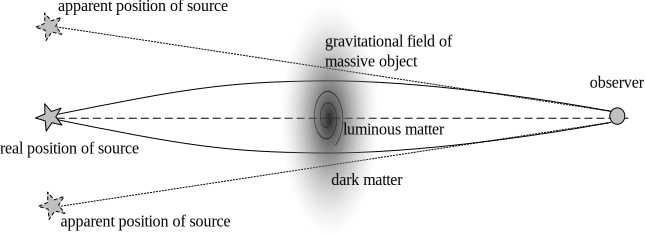
\includegraphics[width=0.75\textwidth]{img/grav_lens}
	\caption{Schematics of gravitational lensing}
	\label{fig:grav_lens}
\end{figure}

This phenomena is divided into three sub categories:
\begin{itemize}
  \item
    \emph{Strong lensing} occurs if the lens is extremely massive. For example single galaxies, galaxy clusters or black holes.
    Strong lensing allows not only for displacements of sources, but also for magnification and creation of multiple images, arc like structure or even rings.
    The first observed strong lensing was the twin quasar Q0957+561 discovered 1979\cite{walsh19790957} and a popular one is the Einstein Cross Q2237+030\cite{ec1985}, shown in Fig.~\ref{fig:einsteinc}.
  \item
    \emph{Weak lensing} phenomena are not directly observable.
    The lensing caused by a weak or far away gravitational field causes only a distortion of the shape of the sources (shear), that can be statistically analysed.
  \item
    \emph{Micro lensing} deals with small perturbations of the perceived light magnitude from a source, caused by a gravitational field in the order of a single lensing star.
    Micro lensing is proposed to be used to detect MACHOs\footnote{Massive Astrophysical Compact Halo Object} and extra solar planets.
\end{itemize}

\begin{figure}[h]
	\centering
		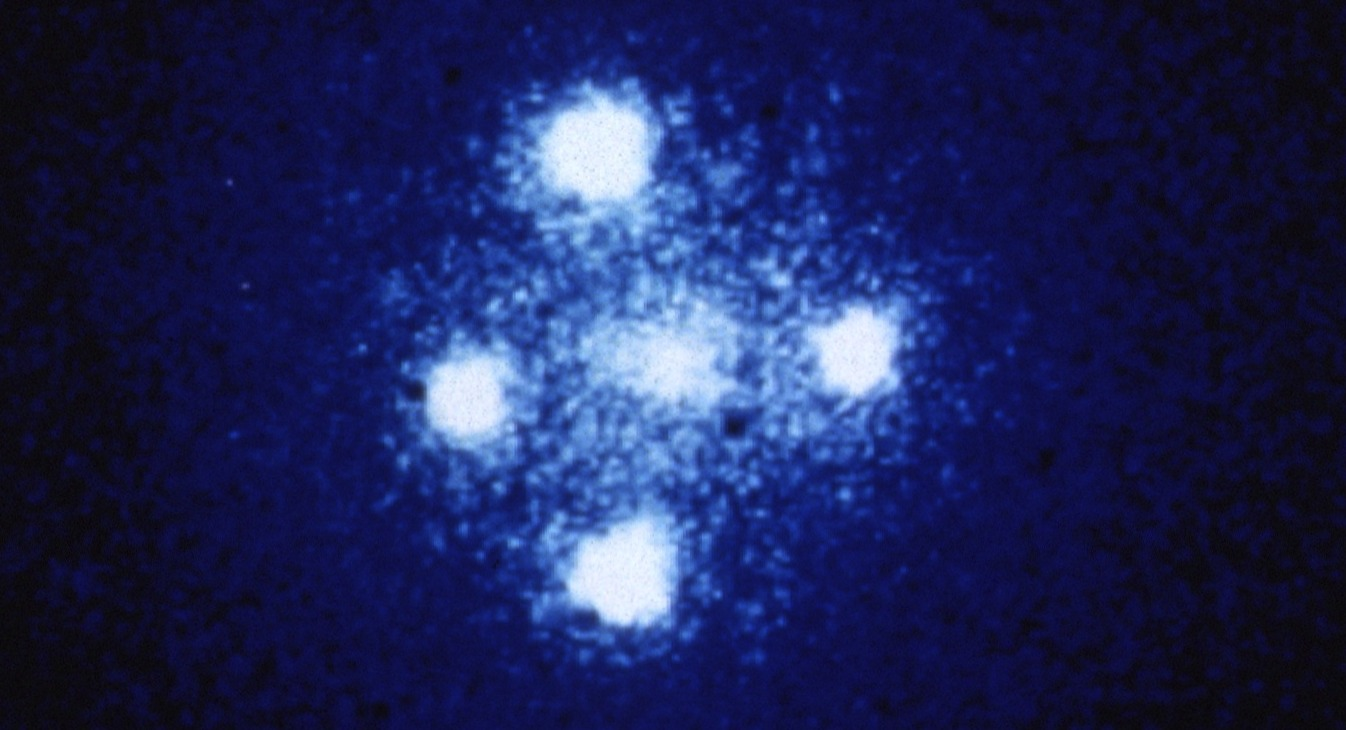
\includegraphics[width=0.5\textwidth]{img/einstein_cross}
	\caption{Einstein cross (Q2237+030): Lensing galaxy cluster in the middle, surrounded by 4 images of the same source quasar, behind the lensing galaxy cluster. (HST; \cite{ec1985})}
	\label{fig:einsteinc}
\end{figure}


\subsubsection{Scientific Relevance of Gravitational Lenses}

The effect of gravitational lensing depends on a variety of cosmological parameters.
Gravitational lenses offer means to estimate many of those parameters.
The study of a discovered gravitational lens usually involves finding the arrangement and properties of the source and the lensing objects.
Simulating these features has to lead to a similar image as the one you see on the telescope.
This process is commonly referred to as \emph{modelling} a gravitational lens.
These models allow to tackle down a lot of open questions in current astrophysics.


A working model of a lens allows to estimate total masses of distant lensing galaxies or clusters.
It takes into account the total mass of the lens (the visible regular matter \emph{and} the dark matter\cite{kochanek1995there}).
Thus it offers an alternative approach\footnote{Alternative to the approach of particle physics using particle colliders.} to tackle down the mystery of dark matter.
It allows to measure the ratio of visible matter to dark matter and the radial distribution of dark matter in galaxies\cite{treukoop04}.
Additionally it allows to test other standard procedures to estimate distant masses\cite{kochanek1995there}.

Looking at sources in a gravitational lensing model provides information about potentially very early objects in the universe.
Those objects can only be observed due to the magnification effect of a lens and these observations could lead to new information about the early evolution of the universe\cite{rusin03}.

If two or more images of the same source can be observed, there is usually a time delay between those images, since the light paths of the two images have different length.
This information can be used to narrow down fundamental cosmological parameters like Hubble time, Lambda constant and cosmological curvature.
This has been described in \cite{refsdal1964} and has recently been used by \cite{age_uni} and \cite{2014MNRAS.437..600S}.


Models are usually produced individually by a scientist using one of the modelling codes available, see \cite{overview_soft2013} for an overview.
This is a time consuming manual process, involving writing script files for modelling software.
For further analyses, like \cite{age_uni}, several models of several lenses need to be combined.

These possibilities of gravitational lenses lead to a high demand for detections of many more lenses and for the ability to model them quickly.



\subsubsection{Detecting Gravitational Lenses}

Today, about 400 secure gravitational lenses have been found and another 200 likely candidates.
Most of these lenses have been found accidentally by researchers looking at astronomical images for other reasons.
Using imagery from Hubble Space Telescope (HST) and current ground based telescopes leads to a detection rate of about 1 lens per 1 to 10 square degrees\footnote{1 square degree $\approx$ 0.03\% of the sky}.

The first systematic surveys for gravitational lenses (DES\footnote{\url{http://www.darkenergysurvey.org}} or PanStarrs\footnote{\url{http://pan-starrs.ifa.hawaii.edu}}) start running these days.
Due to their large survey area and given the current detection rate, they are expected to lead to thousands of new discoveries over the next five years.
In the 2020s, the next generation of surveys (ground based LSST\footnote{\url{http://www.lsst.org}}, space based Euclid\footnote{\url{http://sci.esa.int/euclid/}} and WFIRST\footnote{\url{http://wfirst.gsfc.nasa.gov/}}) are expected to ramp up the detection rate and result in ten thousands of new lenses.

Current surveys cover thousands of square degrees, containing millions of galaxy images that have to be scanned in order to find the rare lenses.
There have been trials with computer algorithms (robots) scanning the huge amount of data and automatically identifying lensing systems\cite{robots}, with mixed results.
They work well in clean lensing systems with no other light sources in the background.
In most situations however, the robots either miss many lenses (low completeness) or identify many other objects as lenses (low purity).
This makes manual inspection indispensable.

Taking these results into account, the \emph{SpaceWarps} project\footnote{\url{http://www.spacewarps.org}} has been started in May 2013, as part of the \emph{Zooniverse} citizen science project\footnote{\url{https://www.zooniverse.org/}} by some of the scientists that were involved with programming robots.
In \emph{Zooniverse}, members of the public (``volunteers'', ``citizen scientists'') are invited to help to analyse different kinds of scientific data that are too difficult to analyse for robots and too excessive for specialists.
SpaceWarps applies this concept to the problem of finding the rare lenses in the huge stack of images produced by the surveys.
Volunteers are asked to scan through the images and mark any possible lenses.
If a configuration has been marked by many volunteers, it gets to the list of candidates.
As of January 2015, there have been ``almost 6 million classifications of images from tens of thousands of people'' that resulted in a list of 3300 lensing candidates for further investigation\footnote{This is not officially published data taken from \url{http://blog.spacewarps.org}}.



\subsection{Own Research}

\subsubsection{Motivation}

The big success of SpaceWarps and the expected exponential increase in detected lenses lead to one problem:
They all have to be modelled in order to be of any scientific use.
Unfortunately, the number of physicists will probably not increase exponentially any time soon.
On the other side, robots still have problems at identifying lenses, they will not be able to produce reliable models for many years.

This leads to the fundamental idea of my work:

{\bf Involve volunteers not only in the process of finding lenses,\\but also in modelling them.}

This involves several steps:

\begin{enumerate}
  \item Improve existing modelling software, make it user-friendly and usable from all operating systems.
  \item Distil the needed knowledge down to easily digestible units understandable by non scientists.
  \item Prove that models generated by volunteers are scientifically relevant.
  \item Find volunteers willing to spend time for the project.
\end{enumerate}

Unlike other projects (like Foldit\footnote{A project solving protein folding problems; \url{http://fold.it}}) I don't intend to make it a game and to hide the scientific aspect.
The project rather offers motivated volunteers new knowledge and an opportunity to learn about and contribute to science.


\subsubsection{Work Already Done - MSc}

I did already start working on the idea to ask volunteers to do gravitational modelling in my MSc thesis and followed it up during the first 8 months of my PhD thesis.

For my MSc thesis\cite{mscth}, I used the existing modelling framework GLASS\cite{glass2, glass} and built a web application around it, called \emph{SpaghettiLens} (SL)\footnote{See \url{http://mite.physik.uzh.ch} and soon \url{http://labs.spacewarps.org/spaghetti}}.
SL makes it easy for volunteers to create, compare, improve and discuss models.
It runs in a web browser, delegating the task to simulate the input to a back-end application server.
For a detailed overview of SL consult my MSc thesis\footnote{\url{http://www.physik.uzh.ch/~rafik/docs/spaghettilens.pdf}}.
The first version of SL has now been running successfully without major problems for more than 18 months and has been used by a few volunteers to generate approximately 2000 models\footnote{The database shows 12'000 entries, most of these are however intermediate results or improvements of previous generated models.} of more than 1000 more or less possible lens candidates from the SpaceWarps catalogue.

%Even though it's still in a testing phase, it is currently running and being used by a few volunteers already
%\footnote{See \url{http://mite.physik.uzh.ch} for SL; \url{http://mite.physik.uzh.ch/data/4516} for a created model.}.
%About 10 volunteers beta testing SL have already generated approximately 2000 models\footnote{The database shows 12'000 entries, most of these are however intermediate results or improvements of previous generated models.} of more than 1000 more or less possible lens candidates from the SpaceWarps catalogue.

The basic idea of SL is to present the to be modelled original survey image on the left hand side, where the user identifies features like lensed images and marks them.\footnote{More precisely, the user has to identify the lensing object, find all the images of the source object and guess their ordering with respect to arrival time.}
That is sufficient to create a model, but professionals could provide more parameters.
In a next step, the user makes the server generate a simulation of the model, based on the user's input.
The model is rendered on the server side and a synthetic image is generated (among other data).
This image is shown on the right hand side and allows visual comparison to evaluate how accurate the model is (depicted in Fig.~\ref{fig:client_screen}).
The user can now improve the model by trying to make the simulated image on the right hand side look like the original survey image on the left hand side by playing around with the input.
At the end of this process, the user can submit the final version of the model.
He receives a link to a summary page\footnote{For example: \url{http://mite.physik.uzh.ch/data/4516}}.
Other users can use this link and try to revise and improve models generated by other users.

\begin{figure}
	\centering
		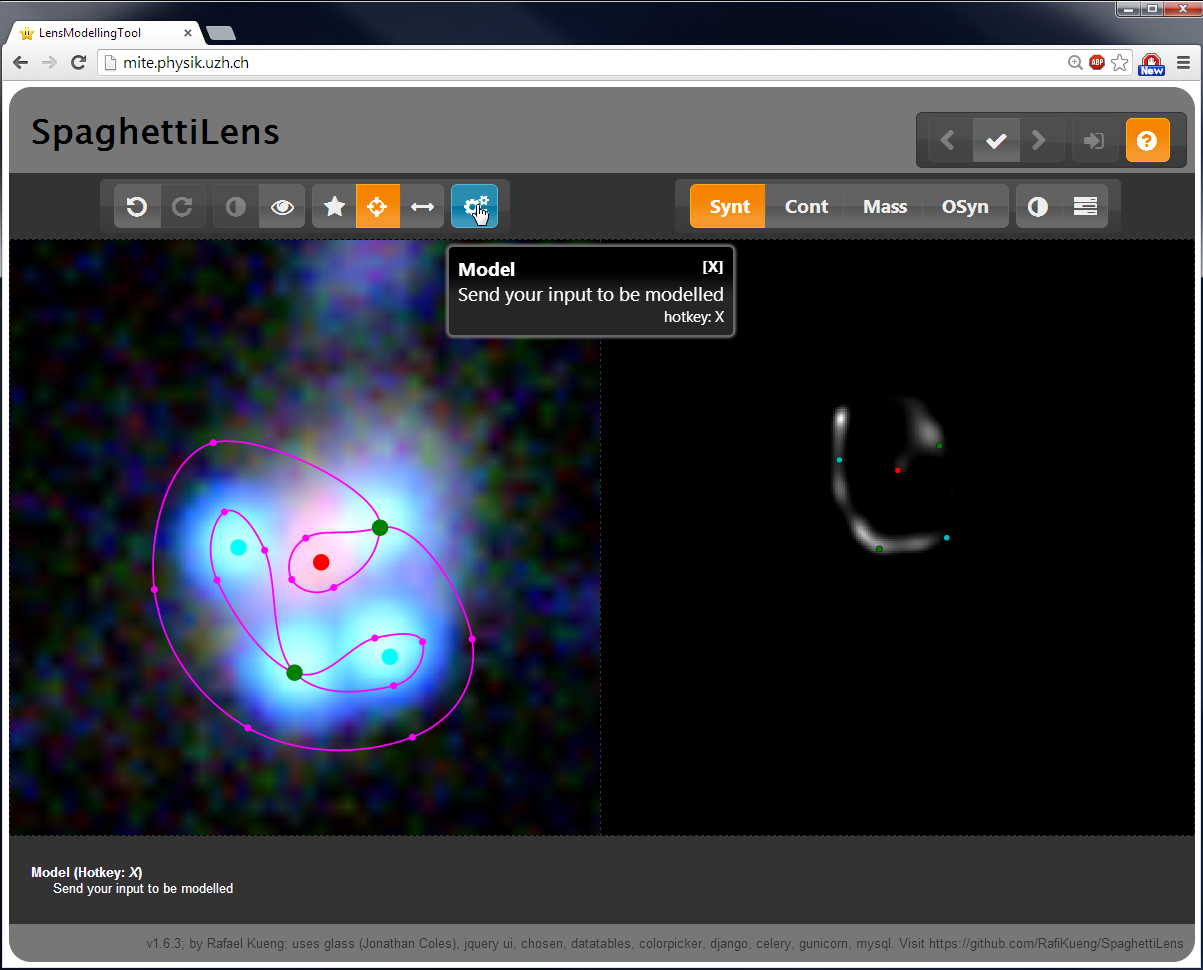
\includegraphics[width=0.75\textwidth]{img/client_screen.png}
	\caption{SpaghettiLens user interface}
	\label{fig:client_screen}
\end{figure}


The idea is that users discuss and compare models among each other and with scientists.
This is currently done on the discussion page of the SpaceWarps project.
This allows the volunteers to gather more experience and knowledge.
Experienced volunteers can help out new users and will be able to get help from scientists for difficult cases.

Some volunteers have published a letter\footnote{\url{http://letters.zooniverse.org/letters/86-collaborative_gravitational_lens_modelling_using_spaghettilens_a_spacewarps_project} (free login required)} at Zooniverse, using SL to collaboratively model a discovered lens candidate.


\subsubsection{Work Already Done - PhD}

While the goal of my MSc project was to address point (1) in the list, we did a follow up with an evaluation of the volunteers performance (3).
The conclusions to this evaluation have recently been accepted by MNRAS, see \cite{spaghetti}.

For the evaluation, a small set of interested volunteers were instructed using a tutorial video and on a personal basis by video con, addressing point (2).
Afterwards we did test their ability to create models by letting them model 29 generated, artificial lenses.
This was done by comparing the parameters used to generate the lenses with the ones recovered by the generated models. Additionally the models made by volunteers were compared with models produced by a scientist.
A few minor problems were identified, but they originate from the design of the program and affected the scientist as well as the volunteers.

Besides writing the paper, the first months of my PhD thesis were spent on improving SL. % updating SL to version 2.0.
Since I've been offered new server hardware, I adjusted the software to the new hardware.
My supervisor and a few other scientists expressed ideas for additional features and functionalities.
To make prototyping and development of those easier, I implemented a series of improvements for SL, like a more modular design and a more flexible database.
One of these ideas, source profile fitting, is basically implemented and will be available in the next few weeks with the launch of \url{http://labs.spacewarps.org}.
A second, a module that allows to do photometry is currently under development and will be ready this summer.





\subsubsection{Personal Motivation}

My personal motivation for this project originates in the fact that this project consists of a good mix of several points:

It is a physics research topic that tries to help to answer some fundamental questions about the universe.
This was the most relevant reason why I studied physics at all and why I chose not to do a streamlined, minimalistic bachelors degree but invested some more time to cover more topics in natural sciences.

It also involves many aspects of informatics and programming, which are some of my hobbies.
It is not just about making an algorithm to perform a bit faster, but is about developing a full scale client server application. It involves a back end simulation program, databases, networks and protocols, client side and user interface programming.

For me, the biggest difference to other projects in physics consists in it involving collaboration not only with other scientists, but also with laymen.
On one side, the requirement that non-experts have to understand what is going on helps not to get lost in details, but to keep the big picture in mind.
I think this helps the public to see into physics, to see what is being researched on and what we spend their taxes for.
On the other side, I can use most of the skills I acquired while working with teenagers as a high school teacher, a job that I did not only to pay for my studies, but because I love to motivate people to approach and master difficult questions.


\subsection{Overview: Ongoing and Planned Research}

I present this request to be able to continue and finish my PhD on this project.
I'm asking for an additional 12 months to get to a total of 32 months of PhD thesis.

As originally planned, the thesis is developing in two parallel directions:

First, on the computational side, the ongoing work on SpaghettiLens and the modelling community.
On one side, work with scientists and volunteers to add new features and improve on existing ones.
As already stated, an improved version of SL is basically finished and will be launched for testing in Feb 2015.
On the other side there is the demand for a central place that helps with all kind of lens modelling questions.
For that reason, we will introduce \url{http://labs.spacewarps.org}, were we intend to create a hub for all people interested in modelling, be it volunteer or scientist.
We plan of hosting and presenting not only SL, but all kinds of modelling tools available for an overview and easy use.
On the same page scientists will be able to get all the available data for all the lenses and models in our database.
A prototype of this hub is already available; the full launch however follows in late Feb to March 2015, probably with the updated version of SL.


In the second, more scientific, parallel running part of my PhD thesis, I use SL to model all currently known lenses by myself.
I will keep up with new discoveries during the thesis period in order to be able to present a complete catalogue of lenses and models at the end of my thesis.
These models will be used at least (i) to study the roles of dark matter and baryons in galaxies and (ii) to identify and prioritize lensed quasars for follow-up time-delay surveys.

The second part will set up an analysis pipeline for models, that will produce scientific relevant data using my own catalogue of models.
If the user base grows as expected, it will be easy to feed those additional models into the analysis pipelines.
This could allow me to compare against the volunteers, or combine the datasets to produce more significant results.
This however is a bonus that depends on factors not entirely under my control.
It will be a nice extra, but it won't be necessary to produce valuable scientific results.

While I haven't done much yet in this part of my thesis, the upgrades to SL already done were essential to allow easy implementation of several complex analysis pipelines.


The next sections contain a more detailed breakdown of the planning of my PhD thesis.


\subsubsection{Work Done (May 2014 - Jan 2015)} \label{sec:plan_done}

\begin{itemize}
  \item Finished and published paper about "Gravitational lens modelling in a citizen science context" \cite{spaghetti}
  \item Prototype of \url{http://labs.spacewarps.org}
  \item Ordering and set-up of new server hardware
  \item Ported SL to new server
  \item Changed database back end for more flexibility
  \item Gathering ideas for photometry and sketching a prototype (on paper)
  \item Completed a working prototype of source profile fitting
  \item Created overview of all modelled lenses
\end{itemize}



\subsubsection{Short Term (Summer 2015)} \label{sec:plan_short}
My first Candoc grant will start in March 2015, running for 10 months.

\begin{itemize}
  \item Increase central resolution (fixes problems identified in \cite{spaghetti}).
  \item Deploy source profile fitting
  \item Develop and deploy photometry module
\end{itemize}



\subsubsection{Mid Term (Winter 2015)} \label{sec:plan_mid}
I'll be able to reach these goals with the first Candoc grant, after one and a half year of PhD thesis.

\begin{itemize}
  \item Write and publish a paper about the findings of the photometry module
  \item Allow modelling of cluster lenses (for researchers/professionals).
  \item Model all known lenses, keep up-to-date with newly discovered lenses.
\end{itemize}



\subsubsection{Long Term (Winter 2016)} \label{sec:plan_long}
If I get the extension grant, I'll be able to finish all my plans listed here and (hopefully) successfully graduate.

\begin{itemize}
  \item Set up all needed analysis pipelines
  \item Have all lens candidates modelled
  \item Publish data obtained from models
  \item Write thesis
\end{itemize}
  
  

\subsection{Resources}

I consider the personal contact to other scientists and volunteers alike as a key component for motivating new volunteers to join the project, to keep participating volunteers motivated and to create a productive atmosphere among scientists and volunteers.
Thus I'm requesting a small budget to travel to conferences and meetings of scientists, to organise get-togethers for volunteers and to organise projects to increase publicity, for example by organising special events for high schools\footnote{I do know from my time as high school teacher that there is a great demand for such events.}. Both the publicity office of the MNF and the physics department showed already interest in supporting such events.

Volunteers joining the project shall do it only because of personal motivation and will never be paid.
Office space and other equipment is already provided by the physics institute.
The new server hardware has been provided by my supervisor.
Thus no further funds are required.





\subsection{Expected Scientific and Broader Impact}

First, this project is essential groundwork for expanding the inventory of lenses and models from currently 400 to a tenfold in five years and maybe 100-fold in ten years.

The inventory of lenses and models will offer scientists the data needed to address some of the currently most pressing questions in physics, like dark matter and the expanding of the universe, among other.
For my thesis, it will offer the opportunity (i) to get a more detailed insight in the roles of dark matter and baryons in galaxies and (ii) to produce a catalogue of lensed quasars for follow up surveys.


%A second problem addressed with my thesis is to establish a network of software, volunteers and researchers to provide the scientific community a fast and reliable way to model large amount of gravitational lenses.
%With upcoming surveys, facilities to analyse and model lenses in large scale will be required.
%We have the opportunity to build up knowledge and infrastructure to make sure the data generated by those missions are properly analysed.

Second, this project will encourage people to participate not simply as anonymous crowd-sources, but as individual citizen scientists.
People will not only get the ability to have an insight in a current leading research field in physics, but also be part of it and contribute personally.

%The side effect of involving the public in science may not be scientifically relevant, but it just might be relevant for science.

\newpage
\bibliographystyle{bib/rplan}
\bibliography{bib/rplan}


\end{document}


